% concatenated from main-isit-2026-opt-clip.tex, prelim.tex, bounding.tex, experiments.tex, conclusion.tex, app-projection.tex
\documentclass[conference,letterpaper]{IEEEtran}
\addtolength{\topmargin}{9mm}
\usepackage{cite}
\usepackage{amsmath,amssymb,amsfonts,amsthm}
\usepackage{ifthen}
\usepackage{tikz}
\usepackage{cite}
\usepackage{url}
\usepackage{titlesec}
\usepackage{subfig}
\usepackage{blkarray}
\usepackage{dsfont}
\usepackage[mathscr]{euscript}
\usepackage{enumitem}
\usepackage{algorithm}
\usepackage[noend]{algpseudocode}
\usepackage{blkarray}
%\usepackage{stfloats}%
%\newtheorem{theorem}{Theorem}
\newtheorem{theorem}{Theorem}[section]
\newtheorem{corollary}{Corollary}[section]
\newtheorem{proposition}{Proposition}[section]
\newtheorem{lemma}{Lemma}[section]
\theoremstyle{remark}
\newtheorem*{remark}{Remark}
\theoremstyle{definition}
\newtheorem{definition}{Definition}[section]
\newtheorem{example}{Example}[section]
%\usepackage{subfig}
\usepackage{subcaption}
\usepackage{blkarray}
\usepackage{dsfont}

\usepackage{url}
\usepackage{tcolorbox}
\usepackage{arydshln}
\usepackage{mathtools}
\usepackage{dsfont}

\usepackage{xcolor}
\newcommand\arv[1]{{\color{red}\textbf{Arvind: #1}}}

\usepackage{xcolor}
\newcommand\anshoo[1]{{\color{blue}\textbf{Anshoo: #1}}}


\definecolor{brickred}{cmyk}{0,0.89,0.94,0.28}
\definecolor{goldenrod}{cmyk}{0,0.10,0.84,0}
\definecolor{purple}{cmyk}{0.45,0.86,0,0}
\definecolor{rawsienna}{cmyk}{0,0.72,1,0.45}
\definecolor{olivegreen}{cmyk}{0.64,0,0.95,0.40}
\definecolor{peach}{cmyk}{0,0.5,0.7,0}
\definecolor{darkolive}{rgb}{0.,0.4,0.}
\colorlet{grey}{gray!40}

\def\tcw{\textcolor{white}}
\def\tcbr{\textcolor{brickred}}
\def \tcbl{\textcolor{blue}}
\def\tcrs{\textcolor{rawsienna}}
\def\tcog{\textcolor{olivegreen}}
\def\tcpl{\textcolor{purple}}
\def\tcgr{\textcolor{grey}}



\global\long\def\P{\mathbb{P}}
\global\long\def\E{\mathbb{E}}
\global\long\def\V{\mathrm{Var}}
\global\long\def\C{\mathrm{Cov}}
\global\long\def\I{\mathbbm{1}}
\global\long\def\d{\mathrm{d}}


\DeclareMathOperator*{\argmax}{arg\,max} \DeclareMathOperator*{\argmin}{arg\,min}  
\DeclareMathOperator*{\Tr}{Tr}
\DeclareMathOperator{\diag}{diag} 
\DeclareMathOperator{\rank}{rank} 
\DeclareMathOperator{\supp}{supp} 

\DeclarePairedDelimiter\ceil{\lceil}{\rceil}
\DeclarePairedDelimiter\floor{\lfloor}{\rfloor} % Use the [cmex10] option to ensure 
\interdisplaylinepenalty=2500

\usepackage[cmintegrals]{newtxmath}
\newlist{mylist}{enumerate}{3}
\setlist[mylist]{label={}}
%\usepackage{algorithmic}
\usepackage{graphicx}
\usepackage{textcomp}
\def\BibTeX{{\rm B\kern-.05em{\sc i\kern-.025em b}\kern-.08em
		T\kern-.1667em\lower.7ex\hbox{E}\kern-.125emX}}

\ifCLASSINFOpdf
\else
\fi

\hyphenation{op-tical net-works semi-conduc-tor}




\begin{document}
\title{Bounding User Contributions for User-Level Differentially Private Mean Estimation}
\author{
	\IEEEauthorblockN{V.~Arvind~Rameshwar}
	\IEEEauthorblockA{Department of Electrical Engineering\\ IIT Madras, Chennai, India\\
		Email: \url{arvind@ee.iitm.ac.in}}
	\and
	\IEEEauthorblockN{Anshoo Tandon}
	\IEEEauthorblockA{IUDX Program Unit\\IISc, Bengaluru, India\\
		Email: \url{anshoo.tandon@gmail.com}}
}
\IEEEoverridecommandlockouts
%\thanks{The authors with the India Urban Data Exchange Program Unit, Indian Institute of Science, Bengaluru 560012, India, email: \texttt{arvind.rameshwar@gmail.com, anshoo.tandon@gmail.com}.}% <-this % stops a 
\maketitle

\begin{abstract}
	We revisit the problem of releasing the sample mean of bounded samples in a dataset, privately, under user-level $\varepsilon$-differential privacy (DP). We aim to derive the optimal method of preprocessing data samples, within a canonical class of processing strategies, in terms of the estimation error. Typical error analyses of such \emph{bounding} (or \emph{clipping}) strategies in the literature assume that the data samples are independent and identically distributed (i.i.d.), and sometimes also that all users contribute the same number of samples (data homogeneity)---assumptions that do not accurately model real-world data distributions. Our main result in this work is a precise characterization of the preprocessing strategy that gives rise to the smallest \emph{worst-case} error over all datasets -- a \emph{distribution-independent} error metric -- while allowing for data heterogeneity. We also show via experimental studies that even for i.i.d. real-valued samples, our clipping strategy performs much better, in terms of \emph{average-case} error, than the widely used bounding strategy of Amin et al. (2019).
\end{abstract}
\section{Introduction}
%Federated learning (FL) is now a widely studied framework for the collaborative training of a machine learning (ML) model by a large collection of devices (also called clients or users), by using decentralized training data. Typically, such a training task proceeds iteratively; in every round, each participating client performs a local update to the machine learning model using its training data and then sends this update to a central server, which is tasked with ``aggregating" the received updates. The aggregated model is then communicated back to the clients, which then begin a fresh round of local model updates. A canonical FL algorithm is the \texttt{FedAvg} algorithm introduced in \cite{fl-mcmahan}. Importantly, FL allows for the training of a large-scale ML model in a distributed fashion, while ensuring that the training data remains private to each client. For a thorough survey of the challenges in real-world deployment of FL, we refer the reader to \cite{kairouz-survey,li-survey}.

In this article, we work on the fundamental problem of processing bounded, potentially vector-valued samples in a dataset, for the release of a private estimate of the sample mean. In particular, we work within the framework of ``user-level" differential privacy \cite{userlevel,hetero}, which is a generalization of the now widely adopted framework of differential privacy (DP) \cite{dworkroth, vadhan2017} for the design and analysis of privacy-preserving algorithms. Loosely, user-level DP guarantees the privacy of a ``user", who could contribute more than one sample, by ensuring the statistical indistinguishability of outputs of the algorithm to changes in the user's samples. User-level DP has practical relevance for inference tasks on real-world datasets, such as traffic datasets, datasets of user expenditures, and time series data, where different users contribute potentially different numbers of samples (data heterogeneity) \cite{usereg3,usereg4}, and more recently, in federated learning (FL) applications (see, e.g., \cite[Sec. 4]{kairouz-survey}). 
%Moreover, user-level DP algorithms are increasingly becoming popular subroutines for integration into
%federated learning (FL) frameworks -- see, e.g., \cite[Sec. 4]{kairouz-survey} for more details. 

%User-level privacy assumes significance in the context of real-world IoT datasets, such as traffic databases, which record multiple contributions from every user (see also \cite{usereg1,usereg2,usereg3,usereg4}). Specifically, user-level DP mechanisms for mean estimation \cite{userlevel,usereg4} are employed by the central server in a canonical FL algorithm such as \texttt{FedAvg} \cite{fl-mcmahan}, while computing a weighted average of gradients passed by each client; these mechanisms help ensure the privacy of a single user (or client), who potentially contributes several samples to the training dataset. 

There are two key requirements of such user-level DP mechanisms for mean estimation. Firstly, the mechanisms must be designed to work with heterogeneous data. Secondly, one would like reliable reconstruction of the true sample mean, even when the data samples are non-i.i.d. (independent and identically distributed). Our focus is hence to  characterize an error metric, which is independent of the underlying data distribution and can be explicitly computed and optimized, for heterogeneous data.

%The second requirement is of particular importance in FL applications, where each client would like to reliably reconstruct the aggregated model update, in every round, from the noisy, privatized aggregate released by the central server, while running the FL algorithm on highly correlated real-world datasets.  

In this article, we confine our attention to user-level (pure) $\varepsilon$-DP algorithms for mean estimation. A key subroutine in such mechanisms \cite{userlevel,hetero-user-level,hist-user-level,amin} is the preprocessing of the data samples for the release of an estimate of the sample mean, which requires the addition of less noise for privacy, as against releasing a noised version of the true sample mean. Such a preprocessing procedure (or ``bounding" or ``clipping" strategy \cite{amin}) either drops selected samples, or projects the samples to a ``high-probability subset". While it is usually easy to establish that such mechanisms are differentially private, an analysis of their ``utility", or the error in estimation of the true statistic, often relies on distributional assumptions about the dataset. 

In this work, following \cite{dp_spcom,dp_preprint,tit-preprint}, we define and explicitly compute the \emph{worst-case error}, over all datasets, of general preprocessing (or bounding) strategies. This error metric is natural in settings with arbitrarily correlated data, where a user potentially ascribes his/her error tolerance to the worst dataset that the statistic is computed on. Furthermore, this error metric is distribution-independent and, as we show, is computable under data heterogeneity too. We then explicitly identify the bounding strategy that results in the smallest worst-case error. Interestingly, we also observe from experimental studies that for scalar samples, our clipping strategy also gives rise to much smaller errors \emph{on average} compared to that in \cite{amin}, for selected dataset sizes, when the samples are drawn i.i.d. according to common distributions.

%In recent work \cite{dp_spcom,dp_preprint,tit-preprint}, the authors introduced the notion of the \emph{worst-case error} incurred by a given mechanism, and showed that such an error metric is explicitly computable for selected clipped, $\varepsilon$-DP estimators for private mean and variance release. Importantly, the worst-case error metric is \emph{independent} of the distribution of the samples in the dataset, and is computable even when the data is heterogeneous. 

%In this work, we generalize the results in \cite{dp_spcom,dp_preprint} by considering clipping strategies that can project or drop data samples, potentially arbitrarily. Our analysis allows us to identify the clipping strategy that results in the smallest worst-case error -- such a strategy simply projects each data sample contributed by a user to an interval determined by the \emph{number} of samples he/she contributes. Our result can be seen as an extension of those in \cite{amin} to the setting of the worst-case error, while allowing for arbitrary bounding strategies. Interestingly, we also observe from experimental studies that our clipping strategy, which does not rely on additional, private parameter estimation unlike that in \cite{amin}, also gives rise to much smaller errors on average as compared to the strategy in \cite{amin}, for selected distributions of numbers of user contributions, when the samples are drawn i.i.d. according to common distributions.

%It is now well-understood that the release of even seemingly innocuous functions of a dataset that is not publicly available can result in the reconstruction of the identities of individuals (or users) in the dataset with alarming levels of accuracy (see, e.g.,  \cite{narayanan, sweeney}). To alleviate concerns over such attacks, the framework of differential privacy (DP) was introduced in \cite{dwork06}, which guarantees the privacy of any single sample. Subsequently, several works (see the surveys \cite{dworkroth, vadhan2017} for references) have designed DP mechanisms for the release of statistics such as the mean, variance, and histograms.




\section{Notation and Preliminaries}
\label{sec:prelim}
\subsection{Notation}
The notation $\mathbb{N}$ denotes the set of positive natural numbers. For $n\in \mathbb{N}$, the notation $[n]$ denotes the set $\{1,2,\ldots,n\}$. 
%An empty product is defined to be $1$. We use the notation $\mathbf{b}$ to denote a vector of predefined length, all of whose symbols are equal to $b\in \mathbb{R}$. 
%Given a real-valued vector $\mathbf{a} = (a_1,a_2,\ldots,a_n)$, we denote its $\ell_1$-norm by $\lVert \mathbf{a} \rVert_1:= \sum_{i=1}^n |a_i|$ and its $\ell_2$-norm by $\lVert \mathbf{a} \rVert_2:= \left(\sum_{i=1}^n a_i^2\right)^{1/2}$. 
%Random variables are denoted by upper-case letters, e.g., $X, Y, \mathbf{Z}$.
%Given a collection of real numbers $(x_1,\ldots,x_n)$, we define its median med$(x_1,\ldots,x_n)$ as any value $x$ such that $|\{i\in [n]: x_i\geq x\}| = \left \lceil n/2\right \rceil$. 
%We write $X\sim P$ to denote that the random variable $X$ is drawn from the distribution $P$. 
Further, given reals $a,b$ with $a\leq b$, we define $\Pi_{[a,b]}(x):= \min\{\max\{x,a\},b\}$, for $x\in \mathbb{R}$. For a vector $\mathbf{x}\in \mathbb{R}^d$, we define its $\ell_p$-norm $\lVert \mathbf{x}\rVert_p$, for an integer $p\in \mathbb{N}$ to be $(\sum_{i=1}^d |x_i|^p)^{1/p}$, with $\lVert \mathbf{x}\rVert_\infty:= \max_{1\leq i\leq d} |x_i|$. For a given set $\mathcal{X}\subseteq \mathbb{R}^d$ and a vector $\mathbf{a}$, we define, with some abuse of notation, $\mathcal{X}(\mathbf{a})$ to be an $\ell_1$-projection $\arg \min_{\mathbf{b}\in \mathcal{X}} \lVert \mathbf{a}-\mathbf{b}\rVert_1$. Given an integer $d\geq 1$ and a real $M\geq 0$, we define $\Delta_M$ to be the $d$-simplex, i.e., $\Delta_M:= \{\mathbf{a}\in \mathbb{R}^d:\ \sum_{i\leq d} a_i\leq M,\ a_i\geq 0,\ \text{for all $i\in [d]$}\}$, and the set $\delta_M:= \{\mathbf{a}\in \mathbb{R}^d:\ \sum_{i\leq d} a_i= M,\ a_i\geq 0,\ \text{for all $i\in [d]$}\}$. Further, for $0\leq \alpha\leq \beta$, we define, with some abuse of terminology, the ``annulus" $\mathsf{A}_{\alpha,\beta}$ as $\mathsf{A}_{\alpha,\beta}:= (\Delta_\beta \setminus \Delta_\alpha) \cup \delta_\alpha$. 

We use the notation $\text{Lap}(b)$ to refer to the zero-mean Laplace distribution with standard deviation $\sqrt{2}b$, the notation $\text{Unif}((0,a])$ to denote the uniform distribution on the interval $(0,a]$, and the notation $\mathcal{N}(\mu, v)$ to denote the Gaussian distribution with mean $\mu$ and variance $v$.

%; its probability distribution function (p.d.f.) obeys
%$$
%f(x) = \frac{1}{2b}e^{-|x|/b}, \ x\in \mathbb{R}.
%$$

%Given a random variable $X$, we denote its variance by $\text{Var}(X)$. The notation ``$\log$'' denotes the natural logarithm.

%and $\mathcal{N}(\mu,\sigma^2)$ to denote the Gaussian distribution with mean $\mu$ and variance $\sigma^2$. For a random variable $X\sim \mathcal{N}(0,1)$, we denote its complementary cumulative distribution function (c.c.d.f.) by $Q$, i.e., for $x\in \mathbb{R}$,
%$
%Q(x):=\Pr[X\geq x] = \int_{x}^{\infty} \frac{1}{\sqrt{2\Pi}} e^{-z^2/2}\d z.
%$
%\subsection{Problem Setup}
%The ITMS dataset that we consider stores records of the data provided by IoT sensors deployed in an Indian city, containing, among other information, the license plate of the bus, the location at which the data was recorded, a timestamp, and the actual data value itself, which is the instantaneous speed of the bus. We process the dataset to extract the data records corresponding to that {h}exagonal ``grid'' in the city {a}nd that {t}imeslot 
%%(we abbreviate \underline{H}exagon \underline{A}nd \underline{T}imeslot  as HAT) 
%which has the highest traffic. 
%We remark that the algorithms discussed in this paper are applicable to general spatio-temporal IoT datasets too. 

\subsection{Problem Formulation}
\label{sec:problem}
Let $L$ be the number of users present in the dataset. For every user $\ell\in [L]$, let the number of records contributed by the user be denoted by $m_\ell$, and set $m^\star:= \max_{\ell\in [L]} m_\ell$ and $m_\star:= \min_{\ell\in [L]} m_\ell$. We assume that $L$ and the collection $\{m_\ell: \ell \in [L]\}$ are known. Now, for a given user $\ell\in [L]$, let $\left\{\mathbf{x}_j^{(\ell)}: j\in [m_\ell]\right\}$ denote the collection of (potentially arbitrary) bounded samples contributed by the user, where each $\mathbf{x}_j^{(\ell)}\in \mathbb{R}^d$, for some dimension $d\geq 1$. We assume, as is common for most applications \cite{dpsgd,dp_spcom}, that {$ \mathbf{x}_j^{(\ell)} \in \Delta_U$}, for all $\ell\in [L]$, $j\in [m_\ell]$, where $U> 0$ is known. Call the dataset as $\mathcal{D} = \left\{\left(\ell,\mathbf{x}_j^{(\ell)}\right): \ell \in [L], j\in [m_\ell]\right\}$.  
%The datasets of interest to us contain samples drawn according to some unknown distribution $P$ that is potentially non-i.i.d. (independent and identically distributed) across samples and users. 

We are interested in releasing the sample mean
\[
	\label{eq:f}
f = f(\mathcal{D}):= \frac{1}{\sum_{\ell'=1}^L m_{\ell'}}\cdot \sum_{\ell=1}^L \sum_{j=1}^{m_\ell} \mathbf{x}_j^{(\ell)}.
\]


%Call the dataset consisting of the speed records of users as $\mathcal{D} = \left\{\left(u_\ell,S_j^{(\ell)}\right): \ell \in [L], j\in [m_\ell]\right\}$, where the collection $\{u_\ell: \ell\in [L]\}$ denotes the set of users. 

%The function that we are interested in computing is the sample average
%$
%f(\mathcal{D}):= \frac{1}{\sum_{\ell=1}^L m_\ell}\cdot \sum_{\ell=1}^L \sum_{j=1}^{m_\ell} S_j^{(\ell)}.
%$

\subsection{Differential Privacy}
\label{sec:dp}
Consider datasets $\mathcal{D}_1 = \left\{\left({\ell},\mathbf{x}_j^{(\ell)}\right): \ell \in [L], j\in [m_\ell]\right\}$ and $\mathcal{D}_2 = \left\{\left(\ell,\overline{\mathbf{x}}_j^{(\ell)}\right): \ell \in [L], j\in [m_\ell]\right\}$ consisting of the same collection of users $[L]$, with each user contributing the same number, $m_\ell$, of  data values. Let $\mathsf{D}$ denote a universal set of such datasets. We say that $\mathcal{D}_1$ and $\mathcal{D}_2$ are ``user-level neighbours'' if there exists $\ell_0\in [L]$ such that $\left(\mathbf{x}^{(\ell_0)}_{1},\ldots, \mathbf{x}^{(\ell_0)}_{m_{\ell_0}}\right)\neq \left(\overline{\mathbf{x}}^{(\ell_0)}_{1},\ldots, \overline{\mathbf{x}}^{(\ell_0)}_{m_{\ell_0}}\right)$, with $\left(\mathbf{x}^{(\ell)}_{1},\ldots, \mathbf{x}^{(\ell)}_{m_{\ell}}\right)$ equal to $ \left(\overline{\mathbf{x}}^{(\ell)}_{1},\ldots, \overline{\mathbf{x}}^{(\ell)}_{m_{\ell}}\right)$, for all $\ell\neq \ell_0$. 
%In this work, we concentrate on mechanisms that map a given dataset to a single real value.

\begin{definition}
	For a fixed $\varepsilon>0$, a mechanism $M: \mathsf{D}\to \mathbb{R}^d$ is  user-level $\varepsilon$-DP if for every pair of user-level neighbours $\mathcal{D}_1, \mathcal{D}_2$ and for every measurable subset $Y \subseteq \mathbb{R}^d$, we have that
	$
	\Pr[M(\mathcal{D}_1) \in Y] \leq e^\varepsilon \Pr[M(\mathcal{D}_2) \in Y].
	$
\end{definition}
%Next, we define the user-level sensitivity of a function of interest.
\begin{definition}
	Given a function $g: \mathsf{D}\to \mathbb{R}^d$, we define its user-level sensitivity $\Delta_g$ as
	$
	\Delta_g:= \max_{\mathcal{D}_1,\mathcal{D}_2\ \text{u-l nbrs.}} \lVert g(\mathcal{D}_1) - g(\mathcal{D}_2)\rVert_1,
	$
	where the maximization is over datasets that are user-level neighbours.
\end{definition}
%For example, the user-level sensitivity of $f$ is
%$\Delta_f = \frac{Um^\star}{\sum_\ell m_\ell}$. 
We use the terms ``sensitivity'' and ``user-level sensitivity'' interchangeably. The next result is well-known \cite[Prop. 1]{dwork06}.

\begin{theorem}
	\label{thm:dp}
	For any $g: \mathsf{D}\to \mathbb{R}^d$, the mechanism $M^{\text{Lap}}_g: \mathsf{D}\to \mathbb{R}$ defined by
	$
	M^{\text{Lap}}_g(\mathcal{D}_1) = g(\mathcal{D}_1)+\mathbf{Z},
	$
	where $\mathbf{Z} = (Z_1,\ldots,Z_d)$ is such that $Z_i\stackrel{\text{i.i.d.}}{\sim} \text{Lap}(\Delta_g/\varepsilon)$, $i\in [d]$, and is independent of $\mathcal{D}$, is user-level $\varepsilon$-DP.
\end{theorem}

\subsection{The Worst-Case Error Metric}

All through, in this paper, we shall work with user-level $\varepsilon$-DP mechanisms that add a suitable amount of Laplace noise that is tailored to the sensitivity of the function used as an estimator of the sample mean $f$. %Now, given any mechanism $M$ for the $\varepsilon$-DP release of $f$, we shall first recall the formal definition of its worst-case error  \cite{tit-preprint}.
Consider a mechanism $M$ for the user-level $\varepsilon$-DP release of the statistic $f$. The canonical structure of $M$ (see \cite[Footnote 1]{staircase}, \cite{opt}) is: $M(\mathcal{D}) = \overline{f}(\mathcal{D})+{\mathbf{Z}},$
%\begin{equation}
%	\label{eq:Mbar}
%	M(\mathcal{D}) = \overline{f}(\mathcal{D})+{\mathbf{Z}},
%\end{equation}
for some estimator $\overline{f}$ of $f$, with user-level sensitivity $\Delta_{\overline{f}}$, with $\mathbf{Z} = (Z_1,\ldots,Z_d)$, with $Z_i\stackrel{\text{i.i.d.}}{\sim} \text{Lap}\left(\Delta_{\overline{f}}/\varepsilon\right)$, $i\in [d]$.  
%The assumption that our mechanisms are \emph{additive-noise} or \emph{noise-adding} mechanisms is without loss of generality, since it is known that every privacy-preserving mechanism can be thought of as a noise-adding mechanism (see \cite[Footnote 1]{staircase} and \cite{opt}). Moreover, under some regularity conditions, for small $\varepsilon$ (or equivalently, high privacy requirements), it is known that Laplace distributed noise is asymptotically optimal in terms of the magnitude of error in estimation \cite{staircase,opt}.


%Note that we work with the class of mechanisms that add Laplace noise tailored to the sensitivities of each grid, individually, since an explicit computation of the user-level sensitivity of the vector $f$ in \eqref{eq:f} (across all grids) is quite hard, thereby implying the necessity of loose bounds on the amount of noise added, when this notion of user-level sensitivity is used.
%Recall, from the discussion preceding Theorem \ref{thm:comp}, that the assumption that the mechanism ${}^gM_\theta$ is Laplace noise-adding is ca.


%Now, consider the mechanism $M_\theta$ that consists of the composition of the mechanisms ${}^gM_\theta$, over $g\in \mathcal{G}$, i.e., $M_\theta = \left({}^gM_\theta:\ g\in \mathcal{G}\right)$. In many settings of interest, a natural error metric for such a composition of mechanisms acting on different grids is the \emph{largest}  \emph{worst-case} estimation error among all the grids. 

For the mechanism $M$, we define its \emph{worst-case} estimation error as
\begin{equation}
	\label{eq:eg}
	E_M = E_{\overline{f}}^{(d)}:= \max_{\mathcal{D}\in \mathsf{D}} \big \lVert f(\mathcal{D}) - \overline{f}(\mathcal{D}) \big\rVert_1 + \E[\lVert{\mathbf{Z}}\rVert_1].
\end{equation}
Clearly, the expression above is an upper bound on the $\ell_1$-error $E^{(1)}_M:= \max_{\mathcal{D}\in \mathsf{D}} \E[|f(\mathcal{D})-M(\mathcal{D})|]$, via the triangle inequality. When the dimension $d$ is clear from the context, we simply denote $E_{\overline{f}}^{(d)}$ as $E_{\overline{f}}$. The distribution-independent expression in \eqref{eq:eg} conveniently captures the errors due to bias (the first term) and due to noise addition for privacy (the second term); a similar such error measure that separates the bias and noise errors was employed in \cite{amin}. 
%and its \emph{worst-case} estimation error over all datasets $\mathcal{D}$ as
%\[
%{}^gE := \max_{\mathcal{D}\in \mathsf{D}} {}^gE(\mathcal{D}).
%\]
%Finally, we define the error metric $E$ of the mechanism $M_\theta$ to be the \emph{largest} worst-case estimation error among all the grids, i.e., $$E := \max_{g\in \mathcal{G}} {}^gE.$$
\section{Worst-Case Errors of Bounding/Clipping Strategies}
\label{sec:bound}
%In this section, we present an explicit characterization of the worst-case errors for a broad class of strategies that work by ``bounding" or ``clipping" the contributions of users, as mentioned in the Introduction. In other words, the estimator $\overline{f}$ of $f$ in \eqref{eq:Mbar} is a suitably clipped or bounded version of the sample mean $f$. We then identify that clipping strategy that leads to the smallest worst-case error.
\subsection{On Clipping Strategies}
We work with estimators $\overline{f} = \overline{f}_{\left\{a_j^{(\ell)},b_j^{(\ell)}\right\}}$ of $f$ obtained by bounding user contributions as follows: for each $\ell\in [L]$ and $j\in [m_\ell]$, we let $\overline{\mathbf{x}}_j^{(\ell)}:= {\mathsf{A}_{a_j^{(\ell)},b_j^{(\ell)}}}\left(\mathbf{x}_j^{(\ell)}\right)$, for reals $0\leq a_j^{(\ell)}\leq b_j^{(\ell)}\leq U$. In words, $\overline{\mathbf{x}}_j^{(\ell)}$ is a projection of $\mathbf{x}_j^{(\ell)}$ onto the set $\mathsf{A}_{a_j^{(\ell)},b_j^{(\ell)}}$ (see Figure \ref{fig:proj}), which, intuitively, reduces the range of values that $\mathbf{x}_j^{(\ell)}$ can take, and hence its sensitivity too. We then set 
\[
\overline{f} = \overline{f}(\mathcal{D}):= \frac{1}{\sum_{\ell'=1}^L m_{\ell'}}\cdot \sum_{\ell=1}^L \sum_{j=1}^{m_\ell} \mathbf{\overline{x}}_j^{(\ell)}.
\]
\begin{figure}
	\centering
	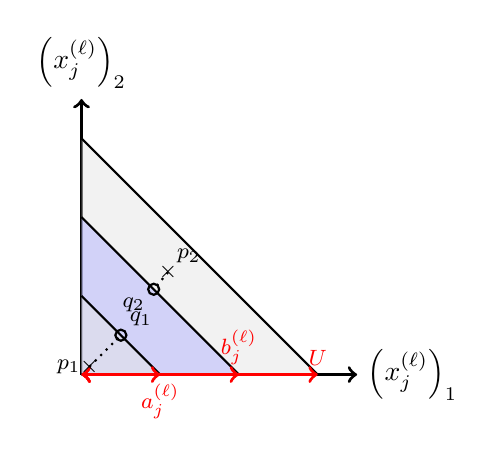
\begin{tikzpicture} [scale=1]% Adjust scale as needed
		
		\newcommand{\outerradius}{3}
		\newcommand{\middleradius}{2}
		\newcommand{\innerradius}{1}
		
		% Draw the axes with new labels (only positive quadrant)
		\draw[->, very thick] (0,0) -- (\outerradius+0.5,0) node[right] {$\left(x_j^{(\ell)}\right)_1$};
		\draw[->, very thick] (0,0) -- (0,\outerradius+0.5) node[above] {$\left(x_j^{(\ell)}\right)_2$};
		
		% Draw the balls with transparency (only positive quadrant)
		\draw[thick, fill=gray!20, fill opacity=0.5] (0,\outerradius) -- (\outerradius,0) -- (0,0);
		
		% Draw the blue region *first* (only positive quadrant)
		\fill[blue!30, fill opacity=0.5] (0,\middleradius) -- (\middleradius,0) -- (0,0);
		
		% Draw the inner ball - make it transparent gray (only positive quadrant)
		\draw[thick, fill=gray!20, fill opacity=0.5] (0,\innerradius) -- (\innerradius,0) -- (0,0); % Inner ball
		
		% Draw the middle ball outline in BLACK (only positive quadrant)
		\draw[thick,black] (0,\middleradius) -- (\middleradius,0) -- (0,0);
		
		\footnotesize
		% Add arrows and labels (red, bold tips)
		\draw[<->, very thick, red, line cap=round] (0,0) -- (\innerradius,0) node [below,font=\footnotesize] {$a_j^{(\ell)}$};
		\draw[<->, very thick, red, line cap=round] (0,0) -- (\middleradius,0) node [above,font=\footnotesize] {$b_j^{(\ell)}$};
		
		\draw[<->,very thick, red, line cap=triangle] (0,0) -- (\outerradius,0) node [above,font=\footnotesize] {$U$};
		
		% Mark the point (0.1, 0.1) and line segment
		\draw[thick, black] (0.1,0.1) node {\textbf{$\times$}} node[left] {$p_1$};
		\draw[dotted, thick] (0.1,0.1) -- (0.5,0.5);
		
		% Calculate the endpoint of the second line segment
		\pgfmathsetmacro{\endx}{1.1/1.2}
		\pgfmathsetmacro{\endy}{1.3/1.2}
		
		% Mark the point (1.1, 1.3)/1.2 with a circle
		\draw[thick, black] (\endx,\endy) circle (2pt) node[below left]{$q_2$};
		
		% Mark the point (1.1, 1.3)
		\draw[thick, black] (1.1,1.3) node {\textbf{$\times$}} node[above right]{$p_2$};
		
		% Draw the dotted line segment from (1.1, 1.3)
		\draw[dotted, thick] (1.1,1.3) -- (\endx,\endy);
		
		% Mark the point (0.5, 0.5) with a circle
		\draw[thick, black] (0.5, 0.5) circle (2pt) node[above right]{$q_1$};
		
	\end{tikzpicture}
	\caption{The annulus $\mathsf{A}_{a_j^{(\ell)},b_j^{(\ell)}}$, for $d=2$, shown in blue. Here, the points $q_1$, $q_2$ equal $\mathsf{A}_{a_j^{(\ell)},b_j^{(\ell)}}(p_1)$ and $\mathsf{A}_{a_j^{(\ell)},b_j^{(\ell)}}(p_2)$, respectively.}
	\label{fig:proj}
\end{figure}
Note that the class $\mathsf{B}$ of estimators $\overline{f}$ as above  captures those estimators obtained by dropping selected samples $\mathbf{x}_j^{(\ell)}$ (by setting $a_j^{(\ell)}= b_j^{(\ell)} = 0$ for those samples) and those obtained by projecting samples onto an $\ell_1$-bounded subset of $\Delta_U$, in addition to strategies that perform a combination of dropping and projection. This class of estimators hence includes several common estimators of the sample mean used in works such as \cite{userlevel,dp_preprint,tit-preprint}.

%In the next subsection, we discuss the worst-case errors (as in \eqref{eq:eg}) of mechanisms that employ some $\overline{f}\in \mathsf{B}$ as the estimator of the sample mean.

\subsection{On Worst-Case Errors of Clipping Strategies}
\label{sec:worst-case}
Consider the quantity $E_{\overline{f}}^{(d)}$, for $\overline{f}\in \mathsf{B}$. The following proposition then holds:
\begin{proposition}
	\label{lem:worst-case}
	We have that
	\begin{align*}
		E_{\overline{f}}^{(1)} \notag&= \frac{1}{\sum_{\ell'\leq L} m_{\ell'}}\cdot \left(\sum_{\ell\leq L}\sum_{j\leq m_\ell} \max\left\{a_j^{(\ell)},U-b_j^{(\ell)}\right\}\right)\ + \notag\\
		&\ \ \  \ \ \ \ \ \ \  \ \ \ \ \ \ \ \  \ \ \ \  \ \ \ \frac{d\cdot\max_{\ell\leq L} \sum_{j\leq m_\ell} \left(b_j^{(\ell)}-a_j^{(\ell)}\right)}{\varepsilon\cdot \sum_{\ell'\leq L} m_{\ell'}}
	\end{align*}
	and for any $d\geq 2$,
	\begin{align*}
		E_{\overline{f}}^{(d)} \notag&= \frac{1}{\sum_{\ell'\leq L} m_{\ell'}}\cdot \left(\sum_{\ell\leq L}\sum_{j\leq m_\ell} \max\left\{a_j^{(\ell)},U-b_j^{(\ell)}\right\}\right)\ + \notag\\
		&\ \ \  \ \ \ \ \ \ \  \ \ \ \ \ \ \ \  \ \ \ \  \ \ \ \ \ \ \ \ \ \ \frac{2d\cdot\max_{\ell\leq L} \sum_{j\leq m_\ell} b_j^{(\ell)}}{\varepsilon\cdot \sum_{\ell'\leq L} m_{\ell'}}.
	\end{align*}
\end{proposition}
The proof of Proposition \ref{lem:worst-case} proceeds with help from a few lemmas. For $E_{\overline{f}}$ as in \eqref{eq:eg}, we define $\beta^{(d)}(\overline{f}) = \beta(\overline{f})$ to be the bias, i.e., $\beta(\overline{f}):= \max_{\mathcal{D}\in \mathsf{D}} \big \lVert f(\mathcal{D}) - \overline{f}(\mathcal{D}) \big\rVert$ and $\eta^{(d)}(\overline{f})=\eta(\overline{f})$ to be the error due to noise addition, i.e., $\eta(\overline{f}):= \E[\lVert\mathbf{\mathbf{Z}}\rVert_1]$. First, we aim to characterize $\beta(\overline{f})$. To this end, we first state a necessary condition for a vector $\mathbf{y}$ to be an $\ell_1$-projection of a vector $\mathbf{a}\in \Delta_U$ onto $\Delta_\alpha$, for $ \alpha\leq U$. 
\begin{lemma}
	\label{lem:proj1}
	Given $\mathbf{a}\in \Delta_U$ and $\alpha\leq U$, we have $\Delta_\alpha(\mathbf{a}) = \mathbf{a}$, if $\mathbf{a}\in \Delta_{\alpha}$. Else, any $\ell_1$-projection $\mathbf{y} = \Delta_\alpha(\mathbf{a})$ must satisfy $\lVert \mathbf{y}\rVert_1 = \alpha$, with $y_i\leq a_i$, for all $i\in [d]$.
\end{lemma}
\begin{proof}
	The first statement in the lemma is clear. Now, for $\mathbf{a}\notin \Delta_\alpha$, suppose that $\mathbf{y} = \Delta_\alpha(\mathbf{a})$ is such that $\lVert \mathbf{y}\rVert_1 < \alpha$. It can then be seen that by setting $\mathbf{y}':= \lambda\mathbf{y}+(1-\lambda)\mathbf{a}$, for some $\lambda\in (0,1)$ such that $\lVert \mathbf{y}'\rVert_1 = \alpha$, we will obtain that $\lVert \mathbf{y}'-\mathbf{a}\rVert_1 < \lVert \mathbf{y}-\mathbf{a}\rVert_1$, which is a contradiction. Likewise, suppose that $y_i>a_i$, for some $i\in [d]$. Now, consider any coordinate $j\in [d]$ such that $y_j\leq a_j$ (such a coordinate must exist, since $\lVert \mathbf{y}\rVert_1 = \alpha$); by letting $m:= \min\{|y_i-a_i|,|y_j-a_j|\}$ and setting $y_i \gets y_i-m$ and $y_j \gets y_j+m$, we see that we strictly decrease $\lVert \mathbf{y}-\mathbf{a}\rVert_1$, which is a contradiction.
\end{proof}
In the appendix, we explicitly characterize the vectors $\mathbf{y}\in \Delta_\alpha$ that are the $\ell_1$-projections of $\mathbf{a}\in \Delta_U\setminus \Delta_\alpha$, for $\alpha\leq U$; indeed, we have that the condition stated in Lemma \ref{lem:proj1} is both necessary and sufficient. The next lemma exactly characterizes the bias $\beta^{(d)}(\overline{f})$, for any $d\geq 1$.
\begin{lemma}
	\label{lem:proj2}
	We have that for any $d\geq 1$,
	\[\beta^{(d)}(\overline{f}) = \frac{1}{\sum_{\ell'\leq L} m_{\ell'}}\cdot \left(\sum_{\ell\leq L}\sum_{j\leq m_\ell} \max\left\{a_j^{(\ell)},U-b_j^{(\ell)}\right\}\right).\]
\end{lemma}
\begin{proof}
	For a sample $\mathbf{x}_j^{(\ell)}\in \mathsf{A}_{a_j^{(\ell)},b_j^{(\ell)}}$, it is clear that $\mathsf{A}_{a_j^{(\ell)},b_j^{(\ell)}}(\mathbf{x}_j^{(\ell)}) = \mathbf{x}_j^{(\ell)}$. Now, suppose that $\mathbf{x}_j^{(\ell)}\in \Delta_U\setminus \Delta_{b_j^{(\ell)}}$. Following Lemma \ref{lem:proj1}, if $\mathbf{y} = \mathsf{A}_{a_j^{(\ell)},b_j^{(\ell)}}(\mathbf{a})$, we must have $$\lVert \mathbf{y} - \mathbf{x}_j^{(\ell)}\rVert_1 = \sum_{i\leq d} ((x_j^{(\ell)})_i - y_i) = \lVert \mathbf{x}_j^{(\ell)}\rVert_1 - b_j^{(\ell)}.$$ Hence, the worst-case clipping error for sample $\mathbf{x}_j^{(\ell)}$ is $$\max\ \lVert \mathsf{A}_{a_j^{(\ell)},b_j^{(\ell)}}(\mathbf{x}_j^{(\ell)}) - \mathbf{x}_j^{(\ell)}\rVert_1 = U-b_j^{(\ell)}.$$ By symmetric arguments, one can show that if $\mathbf{x}_j^{(\ell)}\in \Delta_{a_j^{(\ell)}}\setminus \delta_{a_j^{(\ell)}}$, we must have $$\max\ \lVert \mathsf{A}_{a_j^{(\ell)},b_j^{(\ell)}}(\mathbf{x}_j^{(\ell)}) - \mathbf{x}_j^{(\ell)}\rVert_1 = a_j^{(\ell)}.$$ Thus, overall, we obtain that 
	\begin{equation}\max_{\mathbf{x}_j^{(\ell)}\in \Delta_U} \lVert \mathsf{A}_{a_j^{(\ell)},b_j^{(\ell)}}(\mathbf{x}_j^{(\ell)}) - \mathbf{x}_j^{(\ell)}\rVert_1 = \max\left\{a_j^{(\ell)},U-b_j^{(\ell)}\right\}. \label{eq:maxclip}\end{equation} 
	Now, for any dataset $\mathcal{D}$, recall that
	\begin{align}
		&\lVert f(\mathcal{D})-\overline{f}(\mathcal{D})\rVert_1 \notag\\
		%&=\frac{1}{\sum_{\ell'\leq L} m_{\ell'}}\left\lVert \sum_{\ell\leq L}\sum_{j\leq m_\ell} \left(\mathbf{x}_j^{(\ell)} - \overline{\mathbf{x}}_j^{(\ell)}\right)\right \rVert_1 \notag\\
		&=\frac{1}{\sum_{\ell'\leq L} m_{\ell'}}\left\lVert \sum_{\ell\leq L}\sum_{j\leq m_\ell} \left(\mathbf{x}_j^{(\ell)} - \mathsf{A}_{a_j^{(\ell)},b_j^{(\ell)}}(\mathbf{x}_j^{(\ell)}) \right)\right \rVert_1. \label{eq:cliphelp}
	\end{align}
	Putting together \eqref{eq:maxclip} and \eqref{eq:cliphelp} concludes the proof.
%	It is then easy to see that the bias
%	\begin{align}
%		&\max_{\mathcal{D}\in \mathsf{D}} |f(\mathcal{D})-\overline{f}(\mathcal{D})| \notag\\&= \frac{1}{\sum_{\ell'\leq L} m_{\ell'}}\cdot \left(\sum_{\ell\leq L}\sum_{j\leq m_\ell} \max\left\{a_j^{(\ell)},U-b_j^{(\ell)}\right\}\right). \label{eq:bias}
%	\end{align}
\end{proof}
The calculation of $\eta(\overline{f})$ is quite similar to the proof above, and is captured in Lemma \ref{lem:proj3} below.

\begin{lemma}
	\label{lem:proj3}
	We have that $$\eta^{(1)}(\overline{f}) = \frac{d\cdot \max_{\ell\leq L} \sum_{j\leq m_\ell} \left(b_j^{(\ell)}-a_j^{(\ell)}\right)}{\varepsilon\cdot \sum_{\ell'\leq L} m_{\ell'}}$$
	and for any $d\geq 2$,
	$$\eta^{(d)}(\overline{f}) = \frac{2d\cdot \max_{\ell\leq L} \sum_{j\leq m_\ell} b_j^{(\ell)}}{\varepsilon\cdot \sum_{\ell'\leq L} m_{\ell'}}.$$
\end{lemma}
\begin{proof}
Consider first the case when $d = 1$. Via arguments entirely analogous to that in the proof of Lemma \ref{lem:proj2}, the user-level sensitivity of $\overline{f}$ is
$$
	\Delta_{\overline{f}} = \frac{\max_{\ell\leq L} \sum_{j\leq m_\ell} \left(b_j^{(\ell)}-a_j^{(\ell)}\right)}{\sum_{\ell'\leq L} m_{\ell'}},
$$
since in the worst-case, all samples of a user $\ell$ are changed each from $(a_j^{(\ell)},0,\ldots,0)$ to $(b_j^{(\ell)},0,\ldots,0)$. Next, for any $d\geq 2$, we have via similar arguments that
$$
\Delta_{\overline{f}} = \frac{2\max_{\ell\leq L} \sum_{j\leq m_\ell} b_j^{(\ell)}}{\sum_{\ell'\leq L} m_{\ell'}},
$$
since in the worst-case, all samples of a user $\ell$ are changed each from $(b_j^{(\ell)},0,0,\ldots,0)$ to $(0,b_j^{(\ell)},0,\ldots,0)$.
Using $\E[\lVert \mathbf{Z}\rVert_1] = d\E[|Z_1|] = d\Delta_{\overline{f}} /\varepsilon$ gives us the required result.
\end{proof}
The proof of Proposition \ref{lem:worst-case} then follows directly by putting together Lemmas \ref{lem:proj2} and \ref{lem:proj3}.
%\begin{remark}
%	Via the proof of Lemma \ref{lem:worst-case}, we observe that for a given distribution $\{m_\ell:\ell\in [L]\}$ of user contributions, the dataset $\mathcal{D}$ that gives rise to the largest (or worst-case) error is that where $x_j^{(\ell)} = U$, for all $\ell\in [L]$, $j\in [m_\ell]$. We shall use this observation in the next section when we numerically evaluate the performance of the clipping strategy in \cite{amin} on this ``worst-case dataset".
%\end{remark}


Given the characterization of the worst-case error $E_{\overline{f}}$ as above, we proceed with identifying an estimator $f^\star \in \mathsf{B}$ (equivalently, a bounding strategy) that minimizes $E_{\overline{f}}$, over all $\overline{f}\in \mathsf{B}$. Let $T_\varepsilon$ denote the $\left \lceil \left(\frac{2d}{\varepsilon}\right)\right \rceil^{\text{th}}$-largest value in the collection $\{Um_1,Um_2,\ldots,Um_L\}$; if $\varepsilon<2d/L$, we set $T_\varepsilon = 0$. Our main result is encapsulated in the following theorem:
\begin{theorem}
	\label{thm:opt}
	We have that $f^\star = \overline{f}_{\left\{a_j^{(\ell)},b_j^{(\ell)}\right\}}$ minimizes $E_{\overline{f}}$, where
	$
	a_j^{(\ell)} = \max\left\{\frac{Um_\ell-T_\varepsilon}{2m_\ell},0\right\}\text{ and } b_j^{(\ell)} = \min\left\{\frac{Um_\ell+T_\varepsilon}{2m_\ell},U\right\},
	$
	if $d=1$, and $
	a_j^{(\ell)} = 0\ \text{ and } b_j^{(\ell)} =\min\left\{\frac{T_\varepsilon}{m_\ell},U\right\}
	$, for any $d\geq 2$, for all $\ell\in [L]$ and $j\in [m_\ell]$.
\end{theorem}
Some remarks are in order. First, note that the optimal bounding strategy $f^\star$ clips sample values based only on the number of contributions of each user $\ell\in [L]$. Furthermore, note that the interval of projection is determined by $T_\varepsilon$, which is quite similar in structure to the optimal clipping threshold $T$ in \cite{amin} for item-level DP, which is the (privately estimated) $\left \lceil \left(\frac{2}{\varepsilon}\right)\right \rceil^{\text{th}}$-largest \emph{sample value}.

The proof of Theorem \ref{thm:opt} proceeds with help from the following lemma.
\begin{lemma}
	\label{lem:helper}
	For $d = 1$, there exists an estimator $\overline{f}_{\left\{a_j^{(\ell)},b_j^{(\ell)}\right\}}$ minimizing $E_{\overline{f}}$, which obeys $a_j^{(\ell)}+b_j^{(\ell)} = U$, for all $\ell\in [L]$ and $j\in [m_\ell]$. Furthermore, for $d\geq 2$, an estimator $\overline{f}_{\left\{a_j^{(\ell)},b_j^{(\ell)}\right\}}$ minimizing $E_{\overline{f}}$ must set $a_j^{(\ell)} = 0$, for all $\ell\in [L]$ and $j\in [m_\ell]$.
\end{lemma}
\begin{proof}
	Consider any optimal estimator $\overline{f}_{\left\{a_j^{(\ell)},b_j^{(\ell)}\right\}}$, and suppose that $a_j^{(\tilde{\ell})}+b_j^{(\tilde{\ell})}>U$, for some $\tilde{\ell}\in [L]$ and $j\in [m_{\tilde{\ell}}]$. The proof when we suppose that $a_j^{(\tilde{\ell})}+b_j^{(\tilde{\ell})}<U$, for some $\tilde{\ell}\in [L]$ and $j\in [m_{\tilde{\ell}}]$, is similar, and is omitted. Let $\delta =  (a_j^{(\tilde{\ell})}+b_j^{(\tilde{\ell})})-U$. By setting $b_j^{(\tilde{\ell})}\gets b_j^{(\tilde{\ell})}-\delta$, we observe that $\beta^{(d)}(\overline{f})$ remains unchanged, while $\eta^{(d)}(\overline{f})$ either remains unchanged or strictly decreases by $\delta>0$. Moreover, for $d\geq 2$, note from Proposition \ref{lem:worst-case} that increasing any $a_j^{(\ell)}$ from $0$ to a positive value can only strictly increase $E_{\overline{f}}$.
\end{proof}
Hence, to obtain the explicit structure of an estimator $\overline{f}$ that minimizes $E_{\overline{f}}$, it suffices to focus estimators $\overline{f}_{\left\{a_j^{(\ell)},b_j^{(\ell)}\right\}}$ with $a_j^{(\ell)}+b_j^{(\ell)} = U$, for all $\ell\in [L]$, $j\in [m_\ell]$. Then, for $d=1$, there exists an estimator $f^\star$ minimizing $E^{(1)}_{\overline{f}}$ that satisfies
\begin{equation}
	\label{eq:optsimp1}
	E^{(1)}_{f^\star} = \frac{1}{\sum_{\ell'\leq L} m_{\ell'}}\cdot \left(\sum_{\ell\leq L} S^{(\ell)}+\frac{1}{\varepsilon}\cdot \max_{\ell\leq L} \left(Um_\ell - 2S^{(\ell)}\right)\right),
\end{equation}
where for $\ell\in [L]$, we let $S^{(\ell)}:= \sum_{j\leq m_\ell} a_j^{(\ell)}$, for any given estimator $\overline{f}$. Furthermore, for any $d\geq 2$, there exists an estimator $f^\star$ minimizing $E^{(d)}_{\overline{f}}$ that satisfies
\begin{equation}
	\label{eq:optsimpd}
	E^{(d)}_{f^\star} = \frac{1}{\sum_{\ell'\leq L} m_{\ell'}}\cdot \left(\sum_{\ell\leq L} \overline{S}^{(\ell)}+\frac{2d}{\varepsilon}\cdot \max_{\ell\leq L} \left(Um_\ell - \overline{S}^{(\ell)}\right)\right),
\end{equation}
where for $\ell\in [L]$, we let $\overline{S}^{(\ell)}:= \sum_{j\leq m_\ell} \left(U - b_j^{(\ell)}\right)$, for any given estimator $\overline{f}$. We now prove Theorem \ref{thm:opt}.

\begin{proof}[Proof of Thm. \ref{thm:opt}]
	We prove the theorem in detail for the case when $d=1$; the setting of $d\geq 2$ is quite similar and the proof is hence is omitted. We begin with the expression in \eqref{eq:optsimp1}; note that our task now is simply to identify the optimal parameters $\{S^{(\ell)}:\ \ell\in [L]\}$ of $f^\star$ in \eqref{eq:optsimp1}. Once these parameters are derived, we simply set $a_j^{(\ell)}:= S^{(\ell)}/m_\ell = U-b_j^{(\ell)}$ (via Lemma \ref{lem:helper}), for each $\ell\in [L]$ and $j\in [m_\ell]$. In the expression in \eqref{eq:optsimp1}, let us set $\tau:= \max_{\ell\leq L} \left(Um_\ell - 2S^{(\ell)}\right)$. We hence need to solve the following constrained optimization problem:
	\begin{align}
		&{\text{minimize}}\quad h(\{S^{(\ell)}\}):= \left(\sum_{\ell\leq L} S^{(\ell)}+\frac{\tau}{\varepsilon}\right)\notag\\
		&\text{subj. to:}\ \  Um_\ell-2S^{(\ell)}\leq \tau,\ S^{(\ell)}\geq 0,\ \forall\ \ell\in [L],\ \tau\geq 0.\label{eq:opt}
	%	&\ \ \ \  \ \ \ \  \ \ \ \ \ \ S\geq 0. \label{eq:opt}
	\end{align}
The optimization problem in \eqref{eq:opt} is a linear programming problem. By standard arguments via the necessity of the KKT conditions \cite[Sec. 5.5.3]{boyd}, there must exist reals $\lambda_\tau\geq 0$ and $\lambda_\ell,\ \mu_\ell\geq 0$, for each $\ell\in [L]$ (or Lagrange multipliers), such that the function 
%$$\mathcal{L}(\{S^{(\ell)}\},\ \lambda_\tau,\{\lambda_\ell,\mu_\ell\}):= \sum_{\ell\leq L} S^{(\ell)}+\frac{d\tau}{\varepsilon}-\lambda_\tau \tau\ + \\
%\sum_\ell \lambda_\ell\cdot \left(Um_\ell-2S^{(\ell)}-\tau\right)-\sum_\ell \mu_\ell S^{(\ell)}$$
\begin{align*}
\mathcal{L}(\{S^{(\ell)}\},\ &\lambda_\tau,\{\lambda_\ell,\mu_\ell\}):= \sum_{\ell\leq L} S^{(\ell)}+\frac{S}{\varepsilon}-\lambda_\tau \tau\ + \\
&\sum_\ell \lambda_\ell\cdot \left(Um_\ell-2S^{(\ell)}-S\right)-\sum_\ell \mu_\ell S^{(\ell)}
\end{align*}
obeys the following properties.
\begin{itemize}
	\item \textbf{Stationarity}: We have that $\frac{\partial \mathcal{L}}{\partial \tau} = 0$, or $\lambda_\tau+\sum_\ell \lambda_\ell = \frac{d}{\varepsilon},$
%	\begin{equation}
%		\label{eq:stat1}
%		\lambda_S+\sum_\ell \lambda_\ell = \frac{1}{\varepsilon},
%	\end{equation}
and that $\frac{\partial \mathcal{L}}{\partial S^{(\ell)}} = 0$, for each $\ell\in [L]$, or $\lambda_\ell = \frac{1-\mu_\ell}{2}.$
%\begin{equation}
%	\label{eq:stat2}
%	\lambda_\ell = \frac{1-\mu_\ell}{2}.
%\end{equation}
\item \textbf{Complementary slackness}: We have that $$\lambda_\tau \tau= 0,\ \lambda_\ell\cdot \left(Um_\ell-2S^{(\ell)}-\tau\right) = 0,\ \text{and}\ \mu_\ell S^{(\ell)} = 0,$$
%\begin{align}
%	\label{eq:comp}
%	\lambda_SS = 0,\ \lambda_\ell\cdot \left(Um_\ell-2S^{(\ell)}-S\right) = 0,\ \text{and}\ \mu_\ell S^{(\ell)} = 0,
%\end{align}
for all $\ell\in [L]$.
\end{itemize}
We claim that the assignment $\tau^\star = T_\varepsilon$ and $S^{(\ell),\star} = \max\left\{\frac{Um_\ell-T_\varepsilon}{2},0\right\}$ satisfies the conditions above, for an appropriate choice of $\lambda_\tau,\{\lambda_\ell,\mu_\ell\}$ values. Indeed, for $\ell\in [L]$, if $S^{(\ell),\star} = 0$, we set $\lambda_\ell = 0$ and $\mu_\ell = 1$; else, we set $\lambda_\ell = \frac12$ and $\mu_\ell = 0$. 

%For the setting where $d\geq 2$, the optimization problem \eqref{eq:opt} is modified to the following convex optimization program:
%	\begin{align}
%	&{\text{minimize}}\quad h^{(d )}(\{S^{(\ell)}\}):= \left(\sum_{\ell\leq L} \overline{S}^{(\ell)}+\frac{2d\tau^{(d)}}{\varepsilon}\right)\notag\\
%	&\text{subj. to:}\ \  Um_\ell-2\overline{S}^{(\ell)}\leq \tau^{(d)},\ \overline{S}^{(\ell)}\geq 0,\ \forall\ \ell\in [L], \notag\\
%	&\ \ \ \  \ \ \ \  \ \ \ \ \tau^{(d)}\geq 0. \label{eq:optnew}
%	%	&\ \ \ \  \ \ \ \  \ \ \ \ \ \ S\geq 0. \label{eq:opt}
%\end{align}
%In \eqref{eq:optnew}, we set $\tau^{(d)}:= \max_{\ell\leq L} \left(Um_\ell - \overline{S}^{(\ell)}\right)$. This new optimization problem can be solved similarly using the KKT optimality conditions, to yield the optimal values of $\{a_j^{(\ell)},b_j^{(\ell)}\}$ as in the statement of the theorem.
%An optimal choice of parameters $\{a_j^{(\ell)},b_j^{(\ell)}\}$ of an estimator $f^\star$ thus obeys $a_j^{(\ell)}:= \alpha^{(\ell),\star}/m_\ell = U-b_j^{(\ell)}$, for each $\ell\in [L]$ and $j\in [m_\ell]$.
\end{proof}
Observe that from Theorem \ref{thm:opt}, the optimal worst-case error when $d=1$ is \begin{equation}E^\text{OPT, $(1)$}(\varepsilon)= \frac{1}{\sum_{\ell'\leq L} m_{\ell'}}\cdot\left(\sum_{\ell\leq L} \max\left\{\frac{Um_\ell-T_\varepsilon}{2},0\right\}+\frac{T_\varepsilon}{\varepsilon}\right). \label{eq:eopt1}\end{equation} %
and the the optimal worst-case error for any $d\geq2$ is such that 
\begin{align}& E^\text{OPT, $(d)$}(\varepsilon) \notag\\
	&= \frac{1}{\sum_{\ell'\leq L} m_{\ell'}}\cdot \left( \sum_{\ell\leq L} \max\left\{{Um_\ell-T_\varepsilon},0\right\}+\frac{2dT_\varepsilon}{\varepsilon}\right). \label{eq:eoptd}\end{align} %
%\begin{align}
%&E^\text{OPT}(\varepsilon) \notag\\ &= \frac{1}{\sum_{\ell'\leq L} m_{\ell'}}\cdot\left(\sum_{\ell\leq L} \max\left\{\frac{Um_\ell-T_\varepsilon}{2m_\ell},0\right\}+\frac{1}{\varepsilon}\cdot \min_{\ell\leq L} \{T_\varepsilon,Um_\ell\}\right). \label{eq:erropt}
%\end{align}

%Observe that we have $E^\text{OPT, $(d)$}(\varepsilon) = 2\cdot E^\text{OPT, $(1)$}(\varepsilon)$, for any $d\geq 2$. Note that $T_\varepsilon$ is non-decreasing with $\varepsilon$. The following lemma then holds.
%\begin{lemma}
%\label{lem:monotonicity}
%For any $d\geq 1$, $E^\text{OPT, $(d)$}(\varepsilon)$ is decreasing with $\varepsilon>0$.
%\end{lemma}
%\begin{proof}
%	Via the relationship between $E^\text{OPT, $(1)$}(\varepsilon)$ and $E^\text{OPT, $(d)$}(\varepsilon)$, for any $d\geq 2$, given above, it suffices to prove the lemma for the case when $d=1$. Since $T_\varepsilon = Um^\star$, for all $\varepsilon\geq 2d/L$, it can be seen that $E^\text{OPT}(\varepsilon)$ is indeed non-increasing for $\varepsilon\geq 2d/L$.
%	
%	Now, consider $0<\varepsilon_1<\varepsilon_2<2d/L$; assume for simplicity that we have $m_1\geq m_2\geq \ldots\geq m_L$. Consider the function $g(\varepsilon,t):= \frac{1}{\sum_{\ell'\leq L} m_{\ell'}}\cdot\left(\sum_{\ell\leq L} \max\left\{\frac{Um_\ell-t}{2},0\right\}+\frac{dt}{\varepsilon}\right).$ Then,
%	\begin{align*}
%		E^\text{OPT}(\varepsilon_2)&= g\left(\varepsilon_2,Um_{\left \lceil \left(\frac{2d}{\varepsilon_2}\right)\right \rceil}\right)\\
%		&\leq g\left(\varepsilon_2,Um_{\left \lceil \left(\frac{2d}{\varepsilon_1}\right)\right \rceil}\right)\\
%		&< g\left(\varepsilon_1,Um_{\left \lceil \left(\frac{2d}{\varepsilon_1}\right)\right \rceil}\right) = E^\text{OPT}(\varepsilon_1),
%	\end{align*}
%where the first inequality holds since $t = Um_{\left \lceil \left(\frac{2d}{\varepsilon_2}\right)\right \rceil}$ minimizes $g(\varepsilon_2,t)$, over admissible values of $t$, and the second inequality holds since $\varepsilon_1<\varepsilon_2$.
%\end{proof}
%Hence, we obtain that  $E^\text{OPT}(\varepsilon)$ is monotonically non-increasing as a function of $\varepsilon>0$.
We end this section with a couple of remarks. First, observe from \eqref{eq:eopt1} and \eqref{eq:eoptd} that, in the limit as $\varepsilon\to 0$, the optimal worst-case error equals the worst-case bias error, which in turn equals $U/2$, for $d=1$, and $U$, when $d\geq 2$.

Next, consider the special case of Theorem \ref{thm:opt} when $d=1$, with the interpretation that each sample $x_j^{(\ell)}\in [0,U]$. Here, the annulus $\mathsf{A}_{a_j^{(\ell)},b_j^{(\ell)}}$ is simply the interval $[a_j^{(\ell)}, b_j^{(\ell)}]\subseteq [0,U]$. This implies that for the case when the samples $\mathbf{x}_j^{(\ell)}$ are allowed to take values in the cube $[0,U]^d$, as against in the $\ell_1$-ball $\lVert \mathbf{x}_j^{(\ell)}\rVert_1\leq U$, one can perform the bounding procedure, using the \emph{same} interval $[a_j^{(\ell)}, b_j^{(\ell)}]$ identified via Theorem \ref{thm:opt} for the $d=1$ setting, for each dimension, independently.
	
%
%	\begin{figure}
%		\centering
%		\begin{tikzpicture} [scale=0.8]% Adjust scale as needed
%			
%			\newcommand{\outerradius}{3}
%			\newcommand{\middleradius}{2}
%			\newcommand{\innerradius}{1}
%			
%			% Draw the axes with new labels
%			\draw[->] (-\outerradius-1,0) -- (\outerradius+1,0) node[right] {$(x_j^{(\ell)})_1$};
%			\draw[->] (0,-\outerradius-1) -- (0,\outerradius+1) node[above] {$(x_j^{(\ell)})_2$};
%			
%			% Draw the balls with transparency
%			\draw[thick, fill=gray!20, fill opacity=0.5] (0,\outerradius) -- (\outerradius,0) -- (0,-\outerradius) -- (-\outerradius,0) -- cycle;
%			
%			% Draw the blue region *first*
%			\fill[blue!30, fill opacity=0.5] (0,\middleradius) -- (\middleradius,0) -- (0,-\middleradius) -- (-\middleradius,0) -- cycle;
%	%		\fill[white] (0,\innerradius) -- (\innerradius,0) -- (0,-\innerradius) -- (-\innerradius,0) -- cycle; % "Cut out" the inner part
%			
%			% Draw the inner ball - make it transparent gray
%			\draw[thick, fill=gray!20, fill opacity=0.5] (0,\innerradius) -- (\innerradius,0) -- (0,-\innerradius) -- (-\innerradius,0) -- cycle; % Inner ball
%			
%			% Draw the middle ball outline in BLACK
%			\draw[thick,black] (0,\middleradius) -- (\middleradius,0) -- (0,-\middleradius) -- (-\middleradius,0) -- cycle;
%			
%			\footnotesize
%			% Add arrows and labels (red, bold tips)
%			\draw[<->, very thick, red, line cap=round] (0,0) -- (\innerradius,0) node [below,font=\footnotesize] {$a_j^{(\ell)}$};
%			\draw[<->, very thick, red, line cap=round] (0,0) -- (\middleradius,0) node [above,font=\footnotesize] {$b_j^{(\ell)}$};
%			
%			\draw[<->,very thick, red, line cap=triangle] (0,0) -- (\outerradius,0) node [above,font=\footnotesize] {$U$};
%			
%			
%		\end{tikzpicture}
%		\caption{The annulus is shown in blue.}
%	\end{figure}


\section{Numerical Experiments}
\label{sec:experiments}
In this section, we compare, via numerical experiments, the performance of our clipping strategy for the case when $d=1$, with the widely used strategy in \cite[Sec. 3]{amin}, which we call the ``AKMV" mechanism\footnote{The subscript ``AKMV'' stands for the initials of the last names of the authors of \cite{amin}.}. We straightforwardly adapt the mechanism in \cite{amin} from the item-level setting to the user-level setting, by considering the contribution of a user to be the sum $\sum_{j\leq m_\ell} x_j^{(\ell)}$ of the samples it contributes in the user-level setting. 

%In the first set of experiments, we plot the worst-case error of our clipping strategy against the total estimation error $E_{\text{AKMV}}$, computed via \eqref{eq:eg}, incurred by adapting the clipping strategy proposed in \cite[Sec. 3]{amin} to the setting where users contribute more than one sample to the dataset. 

%\subsection{The Clipping Strategy in \cite{amin}}
%\label{sec:amin}
%We now recall the clipping strategy in \cite[Sec. 3]{amin}. Consider the ``item-level" setting where the dataset $\mathcal{D}'$ is such that each user $\ell\in [L]$ contributes a single sample. Let $\sigma^{(\ell)}$ denote the single sample contributed by user $\ell$. In such a setting, given the fixed collection of positive reals $\{m_\ell: \ell\in [L]\}$ as in Section \ref{sec:problem}, we define the function
%\[
%g = g(\mathcal{D}') = \frac{1}{\sum_{\ell'} m_{\ell'}}\cdot \sum_{\ell=1}^L \sigma^{(\ell)}.
%\]
%Now, in the ``user-level" setting where we are given a dataset $\mathcal{D}$ with numbers of user contributions $\{m_\ell\}$, the function $f$ of interest to us can be viewed as an instance of function $g = g(\mathcal{D}')$ as above, for a dataset $\mathcal{D}'$ where each user $\ell\in [L]$ contributes a single sample. Indeed, by letting $\sigma^{(\ell)}:= \sum_{j=1}^{m_\ell} x_j^{(\ell)}$, we see that the dataset $\mathcal{D}'$ consisting of samples $\{\sigma^{(\ell)}:\ \ell\in [L]\}$ obeys
%$
%f(\mathcal{D}) = g(\mathcal{D}').
%$
%
%Now, in the item-level setting, consider the class $\widehat{\mathsf{B}}$ of estimators $\widehat{g} = \widehat{g}_{T}$ of $g$, paramterized by positive reals $T$. In particular, $\widehat{g}_{T}$ is obtained by letting $\widehat{\sigma}^{(\ell)}:= \Pi_{\left[0,T\right]}\left(\sigma{(\ell)}\right)$, with
%\begin{equation}
%	\label{eq:ghat}
%\widehat{g} = \widehat{g}(\mathcal{D}'):= \frac{1}{\sum_{\ell'=1}^L m_{\ell'}}\cdot \sum_{\ell=1}^L  \widehat{\sigma}^{(\ell)}.
%\end{equation}
%Much like in this work, the authors of \cite{amin} consider the sum of the error due to bias and that due to noise addition for privacy (see \eqref{eq:eg}) as the measure of the total error of a mechanism $\widehat{g}\in \widehat{\mathsf{B}}$. The authors in \cite{amin} then construct an estimator $\widehat{g}$ obtained as follows:
%\begin{enumerate}
%	\item First, parameters $\varepsilon', \varepsilon''$ such that $\varepsilon'+\varepsilon'' = \varepsilon$ are initialized.
%	\item Next, with privacy budget $\varepsilon'$, the $\left \lceil \left(\frac{1}{\varepsilon''}\right)\right \rceil^{\text{th}}$-largest sample among $\{\sigma^{(\ell)}\}$ is estimated and $T$ is set to be this estimate.
%	\item Finally, $\widehat{g}_T$ is released privately by adding noise from the Lap$\left(\frac{T}{\varepsilon''\sum_\ell m_\ell}\right)$ distribution.
%\end{enumerate}
%

Importantly, the AKMV mechanism uses a privacy budget of $\varepsilon/2$ to first \emph{privately} estimate the $\left \lceil \left(\frac{2}{\varepsilon}\right)\right \rceil^{\text{th}}$-largest sample, and then uses this value as the clipping threshold. Via entirely heuristic analysis, the authors of \cite{amin} argue the ``optimality" of AKMV mechanism. However, importantly, their analysis ignores the error in the private estimation of the the $\left \lceil \left(\frac{2}{\varepsilon}\right)\right \rceil^{\text{th}}$-largest sample, rendering such a claim of optimality incorrect. As we shall see, the clipping strategy in \cite[Sec. 3]{amin} performs quite poorly in comparison to our worst-case-error-optimal strategy, in the average case too, when the data samples are drawn i.i.d. from natural distributions.

\subsection{Experimental Setup}
\label{sec:exp-setup}
A natural application of user-level DP mechanisms is to spatio-temporal datasets; similar to previous work \cite{dp_spcom,dp_preprint}, we let $U = 65$, in line with the largest speed of buses in km/hr, in Indian cities. We consider two collections of numbers of user contributions $\{m_\ell:\ \ell\in [L]\}$. 
%We call our first collection loosely as the ``geometric collection", owing to the nature of the distribution of the $m_\ell$ values, and our second collection as the ``extreme-valued collection".
\begin{enumerate}
	\item Geometric collection: Here, we fix an integer $M$ and consider $L = 2^{M+1}-1$ users; for each $i\in \{0,1,\ldots,M\}$, we create $2^i$ users each contributing $2^{M-i}$ samples. 
	%It is clear that there are $2^{M+1}-1$ users overall; further, the total number of samples is $\sum_\ell m_\ell = (M+1)\cdot 2^M$ and $m^\star = 2^M$. 
	In our experiments, we set $M = 6$.
	\item Extreme-valued collection: Here, we consider $L$ users where $L-1$ users contribute one sample each and $1$ user contributes $m^\star>1$ samples. %The total number of samples is $\sum_\ell m_\ell = L-1+m^\star$. 
	In our experiments, we pick $L = 101$, with $m^\star = 10$.
\end{enumerate}
%For a fixed collection $\{m_\ell:\ \ell \in [L]\}$, we recall from the remark following  the proof of Lemma \ref{lem:worst-case}) that the worst-case dataset, i.e., the dataset $\mathcal{D}$ that attains the worst-case error in Lemma \ref{lem:worst-case} is the one where all samples are equal to $U$. 
We also work with the following synthetically generated datasets with i.i.d. samples:
\begin{enumerate}
	\item Uniform samples: Each sample $x_j^{(\ell)}\stackrel{\text{i.i.d}}{\sim} \text{Unif}((0,U])$, across $\ell\in [L]$, $j\in [m_\ell]$. 
	\item Projected Gaussian samples: Each sample $x_j^{(\ell)}$, $\ell\in [L]$, $j\in [m_\ell]$, is drawn i.i.d. by rejection sampling from the $\mathcal{N}(U/2,U/4)$ distribution so that the samples lie in $(0,U]$. 
\end{enumerate}
%\subsection{Performance on the Worst-Case Dataset}
%We first evaluate our clipping strategy and the strategy in \cite[Sec. 3]{amin} on the worst-case dataset. Figure \ref{fig:worst-case} shows the errors incurred by the two strategies on the worst-case dataset. Note that here, we construct the estimator of \cite{amin} by setting $\varepsilon' = \varepsilon'' = \varepsilon/2$ (see Step 1 in Section \ref{sec:amin}) and then executing Step 2 in Section \ref{sec:amin} using (a suitable modification of) the private quantile estimation mechanism in \cite[Algorithm 2]{smith}, to obtain the clipping threshold $T$, as suggested in \cite{amin}. Using the relationship between the user-level setting of interest and a suitably defined item-level setting in Section \ref{sec:amin}, the total estimation error is then calculated via \eqref{eq:eg} as
%\[
%E_{\text{AKMV}} = \frac{1}{\sum_{\ell'} m_{\ell'}}\cdot \sum_{\ell\in [L]} \E\left[\max\{0,Um_\ell-T\}\right]+\frac{2T}{\varepsilon\cdot \sum_\ell m_\ell}.
%\]
%Here, the expectation is over the randomness in the private estimation of $T$. We compute an estimate of $E_{\text{AKMV}}$ above by Monte-Carlo averaging over $10^4$ iterations.
%\begin{figure}[!t]
%	\centering
%	\includegraphics[width = \linewidth]{worst-case-errors.png}
%	\caption{Errors incurred on the worst-case dataset by our clipping strategy and that in \cite[Sec. 3]{amin}}
%	\label{fig:worst-case}
%\end{figure}
%The error of our clipping strategy is computed by plugging in the values of $\{a_j^{(\ell)}\}, \{b_j^{(\ell)}\}$ from Theorem \ref{thm:opt} into the expression in Lemma \ref{lem:worst-case}. From Figure \ref{fig:worst-case}, it is clear that the error incurred by our clipping strategy is much lower that incurred by the strategy in \cite{amin}, for a large range of $\varepsilon$ values. Moreover, the optimal worst-case error is indeed monotonically decreasing with $\varepsilon$, as discussed at the end of Section \ref{sec:worst-case}, as is the (estimate of the) error of the AKMV mechanism on the worst-case dataset.
\subsection{Performance on Synthetic Datasets}
%Given the estimators $f, f^\star, \widehat{g}_T$ as in \eqref{eq:f}, \eqref{eq:fclip}, \eqref{eq:ghat}, respectively, we first put down their sensitivities. Indeed, via straightforward computations, we have that
%\begin{equation}
%	\label{eq:sens1}
%	\Delta_f = \frac{Um^\star}{\sum_\ell m_\ell},\ \Delta_{f^\star} = \frac{\max_\ell \sum_{j\leq m_\ell}(b_j^{(\ell)}-a_j^{(\ell)})}{\sum_\ell m_\ell},\ 
%\end{equation}
%{and}
%\begin{equation}
%	\label{eq:sens2}
%	\Delta_{\widehat{g}_T} = \frac{T}{\sum_\ell m_\ell}.
%\end{equation}
%In \eqref{eq:sens1}, the values $\{a_j^{(\ell)}\}, \{b_j^{(\ell)}\}$ are from Theorem \ref{thm:opt} and in \eqref{eq:sens2}, the threshold $T$ is computed (privately) via Step 2 in Section \ref{sec:amin}.
 
We compare the performances of the following three mechanisms on i.i.d. synthetic datasets:
\begin{enumerate}
	\item the vanilla Laplace mechanism that releases $M_{\text{Lap}}(\mathcal{D}) = f(\mathcal{D})+\mathbf{Z}_1$, where $\mathbf{Z}_1\sim \text{Lap}\left(\frac{\Delta_f}{\varepsilon}\right)$;
	\item the ``OPT-worst-case" mechanism that releases $M_{\text{OPT-wc}}(\mathcal{D}) = f^\star(\mathcal{D})+\mathbf{Z}_2$, where $\mathbf{Z}_2\sim \text{Lap}\left(\frac{\Delta_{f^\star}}{\varepsilon}\right)$; and
	\item the ``AKMV" mechanism \cite[Sec. 3]{amin} that releases $M_{\text{AKMV}}(\mathcal{D}) = \widehat{f}_T(\mathcal{D})+\mathbf{Z}_3$, where $\mathbf{Z}_3\sim \text{Lap}\left(\frac{2\Delta_{\widehat{g}_T}}{\varepsilon}\right)$, and $\widehat{f}_T(\mathcal{D})$ is obtained by clipping the sum of samples of each user to lie in $[0,T]$. Here, $T$ is the estimate of the $\left \lceil \left(\frac{2}{\varepsilon}\right)\right \rceil^{\text{th}}$-largest sample among $\{\sigma^{(\ell)}\}$, which is estimated with privacy budget $\varepsilon/2$.
\end{enumerate}
%\begin{itemize}
%	\item 
%	\item 
%	\item 
%\end{itemize}

The`` average-case" errors on i.i.d. datasets are defined as
$$\overline{E}_\text{Lap} = \E[|\mathbf{Z}_1|],\ \overline{E}_\text{OPT-wc} = \E[|M_{\text{OPT-wc}}(\mathcal{D}) - f(\mathcal{D})|],$$
and
$$ \overline{E}_\text{AKMV} = \E[|M_{\text{AKMV}}(\mathcal{D}) - f(\mathcal{D})|],$$
where the expectations are over the randomness in the data samples and in the DP mechanism employed. These errors 
are then estimated via Monte-Carlo averaging over $10^4$ iterations. As a pre-processing step, we replace each of the samples $\{x_j^{(\ell)}:\ j\in [m_\ell]\}$ of every user $\ell \in [L]$ by the sample average $\frac{1}{m_\ell}\cdot \sum_{j\leq m_\ell} x_j^{(\ell)}$, so as to allow for improved performance post clipping. 

Figure \ref{fig:avg-geo} and \ref{fig:avg-extreme-normal} (with the error axis on a log-scale), respectively, show plots of the (estimates of) the average-case errors for the three mechanisms above for the geometric collection of $\{m_\ell\}$ values and uniform samples, and for the extreme-valued collection with projected Gaussian samples. Interestingly, the average-case performance of the AKMV mechanism is quite similar to, and a little worse than, the average-case performance of the vanilla Laplace mechanism, which in turn is significantly worse than the average-case error incurred by the OPT-worst-case mechanism. A reason for the poor performance of the AKMV mechanism overall is due to the reduced privacy budget allocated to the private release of the clipped estimator. Moreover, in contrast to the OPT-worst-case mechanism, the AKMV mechanism requires the private estimation of the $\left \lceil \left(\frac{2}{\varepsilon}\right)\right \rceil^{\text{th}}$ quantile value, which incurs additional error. We expect that similar trends can be observed for i.i.d. datasets with samples drawn from other distributions of $\{m_\ell\}$ values and samples. We add that while the clipping error remains roughly the same for small changes in $\varepsilon$, there exist certain values of $\varepsilon$ that give rise to sharp discontinuities in the $T_\varepsilon$ values; such behaviour hence results in the (estimates of the) average-case errors not being monotonic in $\varepsilon$, in Figure \ref{fig:avg-geo}.

% Figure \ref{fig:avg-extreme-normal} shows plots of the (estimates of) the average-case errors for the extreme-valued collection of $\{m_\ell\}$ values with projected Gaussian samples. In our experiments, we pick $L = 101$, with $m^\star = 10$, and the errors are shown on a log-scale for easy viewing. These plots show a similar trend in the performances of the three mechanisms as that in Figure \ref{fig:avg-geo}. 
\begin{figure}[!t]
	\centering
	\includegraphics[width = \linewidth]{geo-worst-av-post-av.png}
	\caption{Average-case errors using a geometric collection of $\{m_\ell\}$ values and uniform samples}
	\label{fig:avg-geo}
\end{figure}
%
%\begin{figure}[!t]
%	\centering
%	\includegraphics[width = \linewidth]{avg-extreme-uniform.png}
%	\caption{Average-case errors incurred on a synthetic dataset with an extreme-valued collection of $\{m_\ell\}$ values and uniform samples; here, the errors are shown on a log-scale}
%	\label{fig:avg-extreme-uniform}
%\end{figure}

\begin{figure}[!t]
	\centering
	\includegraphics[width = \linewidth]{extreme-normal-post-av.png}
	\caption{Average-case errors using an extreme-valued collection of $\{m_\ell\}$ values and projected Gaussian samples}
	\label{fig:avg-extreme-normal}
\end{figure}
\section{Conclusion}
\label{sec:conclusion}
In this paper, we revisited the fundamental problem of releasing the sample mean under user-level differential privacy (DP) -- a problem that is well-studied in the DP literature, but typically in the presence of additional (e.g., i.i.d.) assumptions on the distribution of data samples. In our work, we make no distributional assumptions on the dataset; instead, we adopt a worst-case approach to studying the estimation error. We then explicitly characterize this error for a broad class of strategies for bounding user contributions by some combination of clipping the numbers of user contributions and/or clipping the sample values themselves. Our analysis allows us to identify the bounding strategy that is optimal with respect to our worst-case error metric. Via numerical experiments, we demonstrate that our strategy is not only optimal for the worst-case error, but also performs much better than the well-known strategy in \cite{amin} for datasets with i.i.d. samples.

An interesting line of future work will be to extend our worst-case error analysis to the user-level DP release of other statistics, and identify the optimal bounding strategies in those cases as well.

\bibliographystyle{IEEEtran}
{\footnotesize
	\bibliography{references.bib}}
\appendix
\section{Characterizing $\ell_1$-Projections Onto $\Delta_\alpha$}
\label{app:projection}
In this section, we argue that the condition in the second statement of Lemma \ref{lem:proj1} is sufficient for the vector $\mathbf{y}$ to be an $\ell_1$-projection of $\mathbf{a}\in \Delta_U\setminus \Delta_\alpha$, for $\alpha\leq U$.

Following Lemma \ref{lem:proj1}, consider the collection $\mathcal{S}\subseteq \mathbb{R}^d$ of points defined as $\mathcal{S}:= \{\mathbf{z}\in \delta_\alpha:\ z_i\leq a_i,\ \text{for all $i\in [d]$}\}$. Note that  when $a_i>\alpha$, for all $i\in [d]$, we have $\mathcal{S} = \delta_\alpha$. Observe that $\mathcal{S}$ is a convex subset of $\mathbb{R}^d$; hence, by a version of Carath\'eodory's Theorem (see the remark after \cite[Thm. 15.3.5]{cover_thomas} and \cite{carath}), any point $\mathbf{z}$ in $\mathcal{S}$ can be written as a convex combination of finitely many, in particular, $d$ points in $\mathcal{S}$. Hence, consider any such collection $\mathcal{Z} = \{\mathbf{z}_1,\ldots,\mathbf{z}_d\}$ whose convex hull equals $\mathcal{S}$. The following claim then holds.
%Now, consider the case where $\mathbf{a}$ is such that $a_i\leq \alpha$, for some $i\in [d]$, and hence that $a_j\geq \alpha$, for some $j\in [d], j\neq i$.  the proof of the sufficiency of the second statement of Lemma \ref{lem:proj1} for this case is similar to that for the first case, and is omitted.

%For the first case above, consider the collection $\mathcal{Z} = \{\mathbf{z}_1,\ldots,\mathbf{z}_d\}$. Here, for $k\neq i$, we define $\mathbf{z}_k = (z_{k,1},\ldots,z_{k,d})$ to be such that $z_{k,i} = a_i$ and $z_{k,k} = \alpha-a_i$,  with $z_{k,r} = 0$, for $r\notin \{i,k\}$. We define $\mathbf{z}_i = (z_{i,1},\ldots,z_{i,d})$ to obey $z_{i,j} = \alpha$, with $z_{i,r} = 0$, for $r\neq j$. 

\begin{proposition}
	\label{prop:proj1}
	For any $\mathbf{z}\in \mathcal{S}$, we have that $\lVert \mathbf{a} - \mathbf{z}\rVert_1$ is a constant.
\end{proposition}
\begin{proof}
	Recall that by the version of Carath\'eodory's Theorem above, any point $\mathbf{z}\in \mathcal{S}$ can be written as $\mathbf{z} = \sum_{k=1}^d \lambda_k \mathbf{z}_k$, where $\lambda_k\geq 0$, with $\sum_{k\leq d} \lambda_k = 1$.  It suffices to show that $\lVert \mathbf{a} - \mathbf{z}\rVert_1$ is independent of $\{\lambda_k\}$. To see this, note that
	\begin{align*}
		\lVert \mathbf{a} - \mathbf{z}\rVert_1&= \sum_{r\leq d} (a_r-z_r)\\
		&=\sum_{r\leq d} (a_r-\sum_{k\leq d} \lambda_k z_{k,r})\\
		&= \sum_{r\leq d} a_r - \sum_{k\leq d} \lambda_k\cdot \sum_{r\leq d} z_{k,r} = \lVert \mathbf{a}\rVert_1 - \alpha,
	\end{align*}
which is independent of $\{\lambda_k\}$.
\end{proof}
We hence have that the condition in Lemma \ref{lem:proj1} is sufficient for the vector $\mathbf{y}$ in its statement to be an $\ell_1$-projection of $\mathbf{a}$. In practice, given a vector $\mathbf{a}\in \Delta_U\setminus \Delta_\alpha$, one can use the vector $\mathbf{y} = \frac{\alpha}{\lVert \mathbf{a}\rVert_1} \mathbf{a}$ as an $\ell_1$-projection.
%\clearpage
%\appendices
%\section{Proof of Proposition \ref{prop:varsens}}
%\input{app-lem-app1.tex}
%\section{Proof of Theorem \ref{thm:varworst}}
%\input{varworst.tex}
%\section{Experimental Setup}
%\input{app-experiments.tex}
\end{document}
\endinput
%%
%% End of file `sample-sigconf.tex'.
